\documentclass[border=10pt]{standalone}
\usepackage{tikz}\usepackage{amsmath}\usetikzlibrary{arrows.meta}
\begin{document}
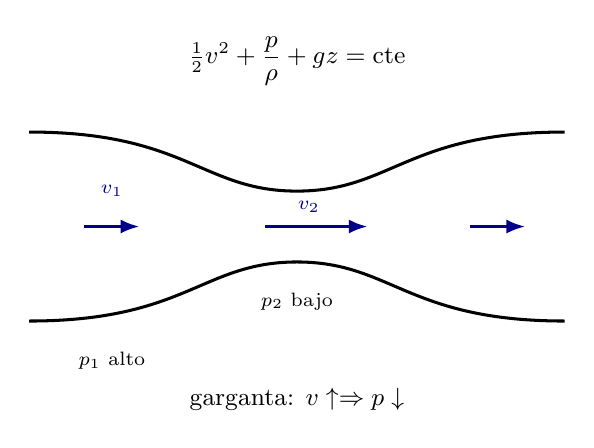
\begin{tikzpicture}[line width=0.9pt,>={Latex[length=2.4mm]}]
  % tubo Venturi (contraccion)
  \draw[line width=1.1pt] (0,1.2) .. controls (2,1.2) and (2.2,0.45) .. (3.4,0.45) .. controls (4.6,0.45) and (4.8,1.2) .. (6.8,1.2);
  \draw[line width=1.1pt] (0,-1.2) .. controls (2,-1.2) and (2.2,-0.45) .. (3.4,-0.45) .. controls (4.6,-0.45) and (4.8,-1.2) .. (6.8,-1.2);
  % velocidad: lenta en ancho, rapida en garganta
  \draw[->,blue!55!black,line width=1.1pt] (0.7,0)--++(0.7,0); \node[blue!55!black] at (1.05,0.45){\scriptsize$v_1$};
  \draw[->,blue!55!black,line width=1.3pt] (3.0,0)--++(1.3,0); \node[blue!55!black] at (3.55,0.25){\scriptsize$v_2$};
  \draw[->,blue!55!black,line width=1.1pt] (5.6,0)--++(0.7,0);
  % presion (manometros)
  \node at (1.05,-1.7){\scriptsize$p_1$ alto}; \node at (3.4,-0.95){\scriptsize$p_2$ bajo};
  \node at (3.4,2.1){\small $\tfrac12 v^2+\dfrac{p}{\rho}+gz=\text{cte}$};
  \node at (3.4,-2.2){\small garganta: $v\uparrow\Rightarrow p\downarrow$};
\end{tikzpicture}
\end{document}
